\documentclass[a4paper, 14pt]{extreport}

\usepackage{vkr}

% Не обязательные библиотеки, используемые только в этом примере:
\usepackage{tikz}
\usetikzlibrary{shadows,arrows}
\usepackage{pgfplots, pgfplotstable}
\pgfplotsset{compat=1.18}
\usepgfplotslibrary{fillbetween}
\usepackage{tikz-dependency}





\begin{document}

\tableofcontents

\bigskip

Набор полезных в написании ВКР примеров и шаблонов.


\section{Простой текст}

Обычный, \textbf{жирный}, \textit{наклонный}, \underline{подчёркнутый} текст. Лучшей практикой будет писать абзац на одной строке: не надо начинать каждое предложение с новой строки или делить текст абзаца ещё как-то. 

Простой список:
\begin{itemize}
    \item раз;
    \item два;
    \item три.
\end{itemize}
Нумерованный список:
\begin{enumerate}
    \item рва;
    \item два;
    \item три.
\end{enumerate}

Можно делать сноски\footnote{Сноска.}.

Имена собственные приводятся на языке оригинала.

\subsubsection{Подраздел}

В ВКР доступны разделы \verb!\section!, подразделы \verb!\subsection! и пункты \verb!\subsubsection!, в крайнем случае подпункты \verb!\paragraph!. Разделы разрешено ставить только в основной части ВКР, во введении, заключении и других структурных элементах ВКР они запрещены. Следует избегать одиночных подразделов и пунктов.

\paragraph{Параграф 1} 

Очень длинный текст.

\paragraph{Параграф 2} Очень длинный текст.




\section{Математика, определения и теоремы}

Математическая формула может стоять в тексте: $E = mc^2$. Для больших формул следует использовать окружение \verb!equation!:
\begin{equation}\label{eq:f1}
    E = mc^2.
\end{equation}
В конце больших формул ставьте подходящий по контексте знак препинания -- это красиво.

На большую пронумерованную формулу можно сослаться: (\ref{eq:f1}), см. раздел \ref{section:references}.

Несколько примеров:

Формула с текстом:
\begin{equation}
    50 \text{ яблок} \times 100 \text{ яблок} =
    \textbf{ много яблок}
\end{equation}

 Различные буквы и шрифты:
\begin{equation}
    \alpha,  \beta,  \gamma, \Gamma, \pi, \Pi, \phi, \varphi, \mu, \Phi, \xi, \zeta;
\end{equation}
\begin{equation}
    \mathbf M, \mathcal C, \mathbb R, \sin \theta = \mathrm{sin} \theta.
\end{equation}

Скобки:
\begin{equation}
    ( a ), [ b ], \{ c \}, | d |, \| e \|, \langle f \rangle, \lfloor g \rfloor, \lceil h \rceil, \ulcorner i \urcorner;
\end{equation}
\begin{equation}
    \left( a + b \right) \left[ 1 - \frac{b}{a+b} \right] = a;
\end{equation}
\begin{equation}
    \sqrt{|xy|} \leq \left| \frac{x + y}{2} \right|;
\end{equation}
\begin{equation}
    \int_a^b u \dv[2]{v}{x} \dd x = \left. u \dv{v}{x} \right|_a^b -\int_a^b \dv{u}{x} \dv{v}{x} \dd x;
\end{equation}
\begin{equation}
    \tilde f(\omega) = \frac{1}{2\pi} \int_{-\infty}^\infty f(x)e^{-i\omega x} \dd x;
\end{equation}
\begin{equation}
    \dot{\vec \omega} = \vec r_c \times \vec I;
\end{equation}
\begin{equation}
    u = \frac{-y}{x^2 + y^2}, \quad v = \frac{x}{x^2 + y^2}, \quad \text{и} \quad w = 0.
\end{equation}

Последовательности:
\begin{equation}
    (1+x)^n = \sum_{i=0}^n \binom{n}{i} x^i;
\end{equation}
\begin{equation}
    e^x = 1 + x + \frac{x^2}{2} + \frac{x^3}{6} + \cdots = \sum_{n \ge 0} \frac{x^n}{n!};
\end{equation}

Дроби:
\begin{equation}
    x = 
    a_0 + \frac{1}{a_1 + \frac{1}{a_2 + \frac{1}{a_3 + a_4}}}
    =
    a_0 + \frac{1}{\displaystyle a_1
        + \frac{1}{\displaystyle a_2
        + \frac{1}{\displaystyle a_3 + a_4}}}.
\end{equation}

Матрицы:
\begin{equation}
    \begin{pmatrix}
        1 & x & 0 \\
        0 & 1 & -1
    \end{pmatrix}
    \begin{pmatrix}
        1  \\
        y  \\
        1
    \end{pmatrix}
    =
    \begin{pmatrix}
        1 + xy  \\
        y - 1
    \end{pmatrix},
    \quad\quad
    \left(
    \begin{matrix}
        2 & 3 & 4\\
        5 & 6 & 7\\
        8 & 9 & 10
    \end{matrix}
    \right)
    v = 0;
\end{equation}
\begin{equation}
    \frac{n!}{k!(n-k)!} = \binom{n}{k};
\end{equation}
\begin{equation}
    \deg A =
    \left|
    \begin{matrix}
        -2 & 1 & 0 & 0 & \cdots & 0  \\
        1 & -2 & 1 & 0 & \cdots & 0  \\
        0 & 1 & -2 & 1 & \cdots & 0  \\
        0 & 0 & 1 & -2 & \ddots & \vdots \\
        \vdots & \vdots & \vdots & \ddots & \ddots & 1  \\
        0 & 0 & 0 & \cdots & 1 & -2
    \end{matrix}
    \right|.
\end{equation}

Фигурная скобка для нескольких случаев:
\begin{equation}
    |x| =
    \begin{cases}
        x, & x \ge 0, \\
        -x, & x< 0.
    \end{cases}
\end{equation}

Формулы в несколько строк:
\begin{align*}
    F &= \{ F_{x} \in F_{c} \mid (|S| > |C|) \\
      &\wedge (\mathrm{minPixels} < |S| < \mathrm{maxPixels}) \\
      &\wedge (|S_{\mathrm{conected}}| > |S| - \epsilon) \}
\end{align*}
или
\begin{multline}
    A_0 = \frac{1}{(\alpha + t_x)^{r + s + x}}{}_2 F_1 \left( r + s + x, x + 1; r + s + x + 1; \frac{\alpha - \beta}{\alpha + t_x} \right) \\
    \quad - \frac{1}{(\alpha + T)^{r + s + x}}{}_2 F_1 \left( r + s + x, x + 1; r + s + x + 1; \frac{\alpha - \beta}{\alpha + T} \right).
\end{multline}

Логика, доказательства:
\begin{equation}
    (\forall \varepsilon > 0) (\exists N \in \mathbb Z^+) (\forall n \ge N) (|x_n - a| < \varepsilon \iff \lim_{n \to +\infty} x_n = a);
\end{equation}
\begin{equation}
    A \implies B, \quad A \iff B, \quad A = \{z \in \mathbb Z \mid z = \bar z \};
\end{equation}
\begin{equation}
    f: X \to Y, \quad f: x \overset{F}{\mapsto} 5x \cos(\tfrac{\pi x}{2})
\end{equation}
\begin{equation}
    \frac{\cancel{\sqrt 2} \sin(x + 2)}{\cancel{2 \cdot \cos(\sfrac{\pi}{4})} \sin(x)} = \frac{\sin(x + 2)}{\sin(x)}, \quad \cancelto{0}{\sin(0)} \equiv 0.
\end{equation}

\newpage
Определения, теоремы:
\begin{Df}[Метрическое пространство]\label{df:example}
    Метрическим пространством называют пару $(S; \rho)$, где для функции-\textit{метрики} $\rho: S \to \mathbb R^+$, если верно следующие три условия:
    \begin{enumerate}
        \item $a \in S : \rho(a, a) = 0$,
        \item $a, b \in S : \rho(a, b) = \rho(b, a)$,
        \item $a, b, c \in S : \rho(a, b) + \rho(b, c) \ge \rho(a, c)$.
    \end{enumerate}
\end{Df}


\begin{Th}[Хаусдорф]\label{th:example}
    В полном метрическом пространстве множество является компактом тогда и только тогда, когда оно замкнуто и вполне ограничено.
\end{Th}
\begin{proof}
    Текст доказательства.
\end{proof}

\begin{Ex}
    Множество вещественных чисел $\mathbb R$ с заданной на нём метрикой $\rho(a, b) = |a - b|$ формируют метрическое пространство.
\end{Ex}
\begin{proof}
    Следует из определения \ref{df:example}.
\end{proof}




\section{Картинки и таблицы}

Используйте окружение \verb!figure! для создания картинок. Код ниже весьма стандартен и его следует копировать каждый раз, когда необходимо вставить новую картинку.

Команда \verb!\includegraphics!, находящаяся внутри внутри окружения, непосредственно вставляет картинку, единственный её аргумент -- путь до картинки. Используйте параметр \verb!scale! для изменения размера картинки. Команда \verb!\caption! задаёт подпись под картинкой. Команда \verb!\label! задаёт уникальные идентификатор объекта, при помощи которого на картинку потом можно ссылаться.

\begin{figure}[h]
    % Выровнение по центру:
    \centering 
    % Параметр scale отвечает за размер картинки:
    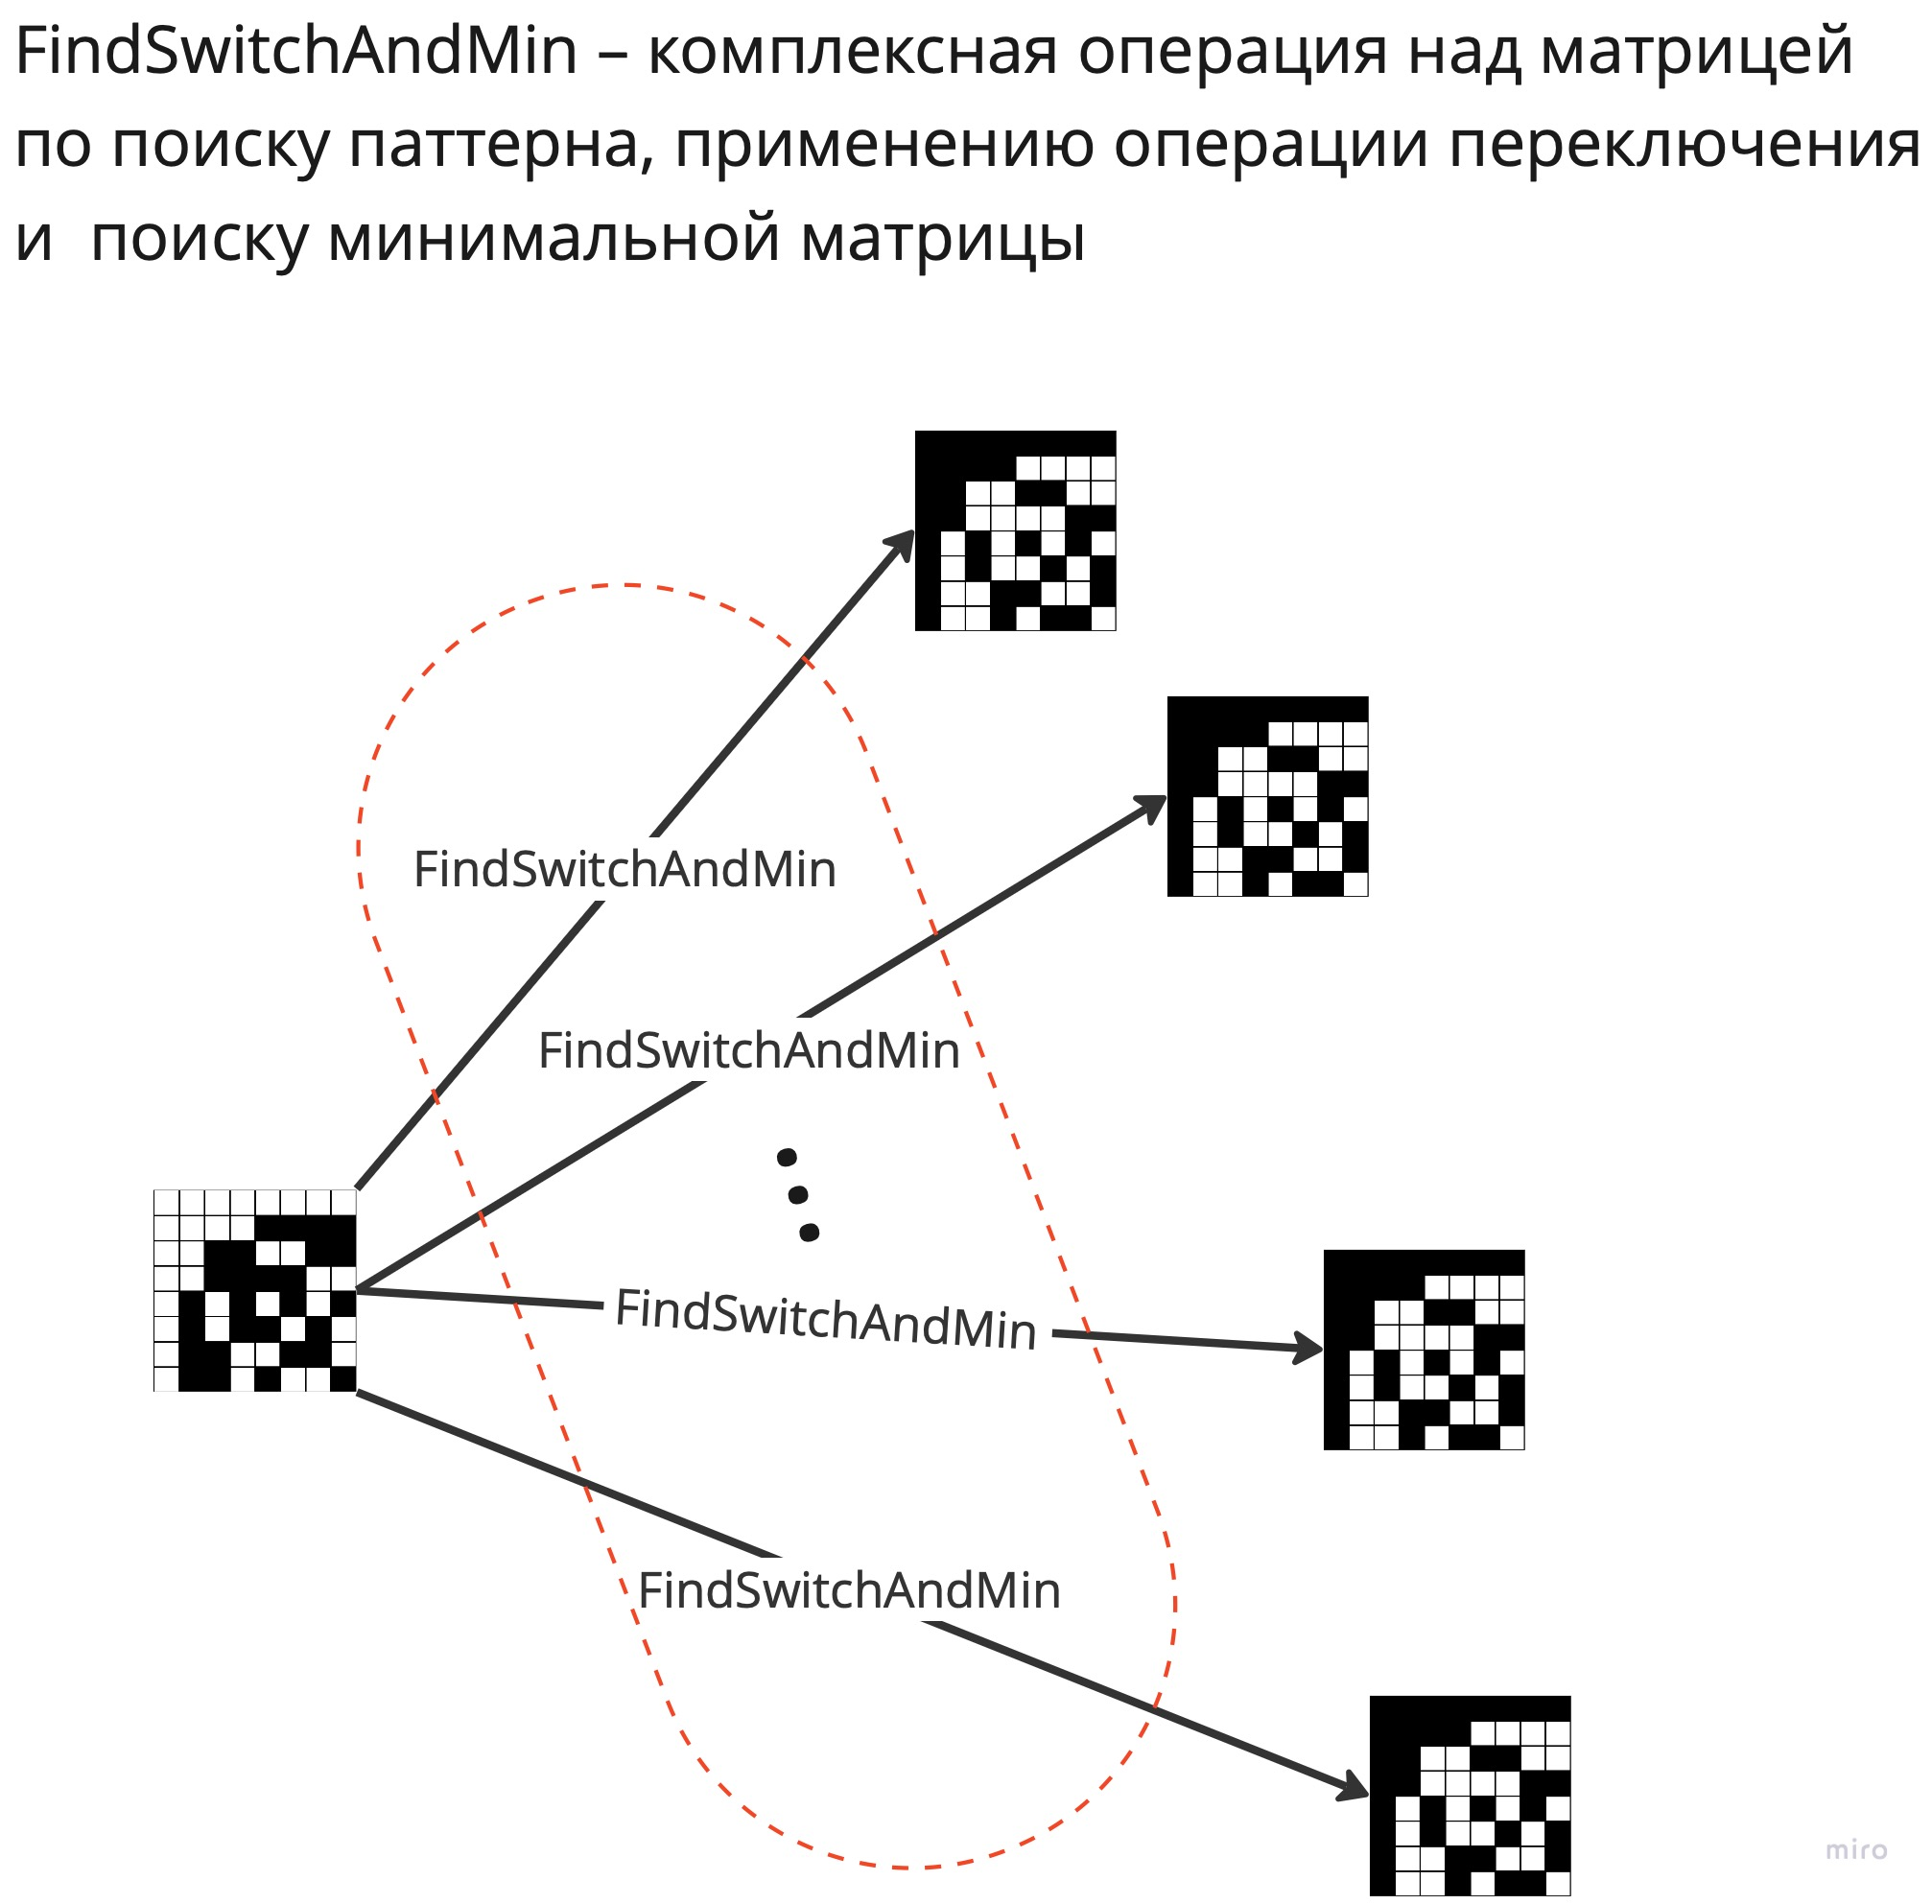
\includegraphics[scale=0.25]{img/graph.jpg}
    % Подпись:
    \caption{Подпись картинки.}
    % Уникальный идентификатор:
    \label{fig:example fig 1}
\end{figure}

Компилятор тех-а сам определяет куда вставлять картинку. Можно <<попросить>> вставить её ближе к тому месту, где находится её код, использовав параметр \verb!h! у самого окружения: в таком случае, картинка будет вставлена в середине текста, так что бы это было красиво, но не обязательно в том месте где стоит её код. Если необходимо иметь картинку конкретно в нужном месте, используется параметр \verb!h! (см. рис. \ref{fig:example fig 2}), однако злоупотреблять такой возможностью не рекомендуется. Если ни одного из этих аргументов нет, картинка почти всегда окажется сверху страницы -- это стандарт для научных статьей.

Исторически сложилось, что таблицы отделяются от картинок, и для них есть отдельное окружение \verb!table!, полностью аналогичное \verb!figure!. Сами таблицы формируются в окружении \verb!tabular!, как в примере ниже. Смотрите \url{https://www.overleaf.com/learn/latex/Tables} для информации по продвинутым таблицам, они не сложные.

\begin{table}[h]
    % Выравнивание по центру:
    \centering 
    % Аргумент lc|r означает три колонки. В первый выравнивание налево (left), во второй выравнивание по центру (center), в третьей выравнивание направо (right). Причём последние две колонки отделены чертой:
    \begin{tabular}{lc|r}
        \textbf{текст} & $1$ & $\alpha$ \\
        \hline % -- горизонтальная черта
        текст & $1$ & $\beta$ \\
        \textit{текст} & $1$ & $\gamma$ \\
    \end{tabular}
    % Подпись:
    \caption{Подпись таблицы.}
    % Уникальный идентификатор:
    \label{fig:example fig 2}
\end{table}

В общем случае, вместо \verb!\includegraphics! в окружении \verb!figure! может стоять любой код. Многочисленные библиотеки позволяют нарисовать большое разнообразие картинок, схем и прочего, используя теховские команды. В некоторых случаях это предпочтительнее чем вставлять иллюстрацию, созданную в сторонней программой, главным образом потому что получающееся в техе изображение -- векторное, и потому не будет падать в качестве при приближении. В сути есть большой набор разнообразных примеров собранных внутри теха картинок: \url{https://texample.net/tikz/examples/}. Однако, всё это по желанию, разумеется. Примеры моих собственных работ ниже:

\begin{figure}[H]
    \centering
    \resizebox{0.5\textwidth}{!}{
        \begin{tikzpicture}[scale=0.9,transform shape]
        
            % Слои:
            \pgfdeclarelayer{background}
            \pgfdeclarelayer{foreground}
            \pgfsetlayers{background,main,foreground}
            
            % Стили:
            \tikzstyle{materia}=[draw, fill=blue!20, text centered,
            minimum height=1.5em,drop shadow]
            \tikzstyle{practica} = [materia, minimum width=10em,
            minimum height=3em, rounded corners, drop shadow]
            \tikzstyle{texto} = [above, text width=10em, text centered]
            \tikzstyle{linepart} = [draw, thick, color=black!50, -latex', dashed]
            \tikzstyle{line} = [draw, thick, color=black!80, -latex']
            \tikzstyle{ur}=[draw, text centered, minimum height=0.01em]
            
            \newcommand{\blockdist}{1.3}
            \newcommand{\edgedist}{1.5}
    
            \newcommand{\practica}[3]{node (p#1) [practica,#3] {#2}}
    
            % Задний фон:
            \newcommand{\background}[5]{%
            \begin{pgfonlayer}{background}
                \path (#1.west |- #2.north)+(-0.5,0.5) node (a1) {};
                \path (#3.east |- #4.south)+(+0.5,-0.25) node (a2) {};
                \path[fill=yellow!20,rounded corners, draw=black!50, dashed]
                (a1) rectangle (a2);
                \path (a1.east |- a1.south)+(1,-0.4) node (u1)[texto]
                {\small~\textit{#5}};
            \end{pgfonlayer}}
    
            \newcommand{\transreceptor}[3]{%
            \path [linepart] (#1.east) -- node [above]
                {\scriptsize Transreceptor #2} (#3);}
            
            % Прямоугольники:
            \path \practica {1}{Изучение задачи}{text width=8.0em,fill=green!30};
            \path (p1.south)+(-0,-1.25) \practica {10}{Построение алгоритма на основе\\ синтаксического дерева}{text width=22.0em,fill=green!30};
            
            \path (p10.south)+(-3,-2.5) \practica{c1}{Использование стороннего синтаксического анализатора}{text width=8.0em};
            \path (p10.south)+(3,-2.1) \practica{m1}{Реализация\\ морфологического анализатора}{text width=8.0em};
            
            \path (pc1.south)+(0,-1) \practica{c2}{Корпус\\ кореференций}{text width=8.0em};
            \path (pm1.south)+(0,-1) \practica{m2}{Морфологический словарь}{text width=8.0em};
            
            \path (pc2.south)+(0,-1) \practica{c3}{Поиск именных\\ групп}{text width=8.0em};
            \path (pm2.south)+(0,-1.4) \practica{m3}{Получение парадигм и аффиксов}{text width=8.0em};
            
            \path (pc3.south)+(0,-1) \practica{c4}{Фильтр \\антецедентов}{text width=8.0em};
            \path (pm3.south)+(0,-1) \practica{m4}{Реализация разбора слова}{text width=8.0em};
            
            \path (pc4.south)+(0,-1) \practica{c5}{Реализация \\нейронной сети}{text width=8.0em};
            \path (pm4.south)+(0,-1) \practica{mend}{Анализ\\ результатов}{text width=8.0em,fill=green!30};
            
            \path (pc5.south)+(0,-1) \practica{cend}{Анализ\\ результатов}{text width=8.0em,fill=green!30};
                
            % Стрелки:
            \path [line] (p1.south) -- node [above] {} (p10);
    
            \path [line] (p10.south)+(-3,0) -- +(-3,-1);
            \path [line] (p10.south)+(3,0) -- +(3,-1);
    
            \path [line] (pc1.south) -- +(0,-0.25);
            \path [line] (pc2.south) -- +(0,-0.25);
            \path [line] (pc3.south) -- +(0,-0.25);
            \path [line] (pc4.south) -- +(0,-0.25);
            \path [line] (pc5.south) -- +(0,-0.25);
            
            \path [line] (pm1.south) -- +(0,-0.25);
            \path [line] (pm2.south) -- +(0,-0.25);
            \path [line] (pm3.south) -- +(0,-0.25);
            \path [line] (pm4.south) -- +(0,-0.25);
            
            \background{pc1}{p1}{pm1}{p10}{Подготовка}
            \background{pc1}{pc1}{pcend}{pcend}{~Кореференция}
            \background{pm1}{pm1}{pmend}{pcend}{Морфология}
        \end{tikzpicture}
    }
    \caption{Пример схемы исследования. Картинка равномерно уменьшена чтобы занимала меньше места.}
    \label{fig:example fig 3}
\end{figure}

\begin{figure}[H]
    \centering\footnotesize
    \resizebox{0.9\textwidth}{!}{
        \begin{tikzpicture}
        
        \tikzstyle{layer}=[rectangle,rounded corners,line width=1pt,draw=black,fill=white,minimum size=20pt,inner sep=0pt]
        \tikzstyle{neuron}=[circle,line width=1pt,draw=black,fill=white,minimum size=14pt,inner sep=0pt]
        \tikzstyle{warrow}=[->, line width=1pt]
            
            \def\layercen{5.225}
            \def\layerY{-\i*1.6}
            \def\layerCY{\layerY-0.2}
            \def\layersOffset{2}
            \def\layerUpperTextA{Итоговая оценка $\mathbf r_n$}
            \def\layerUpperTextB{Скрытый слой $\mathbf h_3$}
            \def\layerUpperTextC{Скрытый слой $\mathbf h_2$}
            \def\layerUpperTextD{Скрытый слой $\mathbf h_1$}
            \def\layerUpperTextE{Входной слой $\mathbf h_0$}
            \def\layerBottomTextA{Эмбэддинг\\и контекст\\антецедента}
            \def\layerBottomTextB{Признаки\\антецедента}
            \def\layerBottomTextC{Эмбэддинг\\и контекст\\постецедента}
            \def\layerBottomTextD{Признаки\\постецедента}
            \def\layerBottomTextE{Признаки\\пары}
            
            \def\treedots#1{
                \node[circle,fill=black,minimum size=3pt,inner sep=0pt, right=of #1, xshift=-5.75ex] {};
                \node[circle,fill=black,minimum size=3pt,inner sep=0pt, right=of #1, xshift=-4.50ex] {};
                \node[circle,fill=black,minimum size=3pt,inner sep=0pt, right=of #1, xshift=-3.25ex] {};
            }
            
            \def\vectorTypeA#1#2#3{
                \node[anchor=west,layer,minimum width=3.8cm,#2, minimum height=0.8cm] (layer) at (#1, \layerCY) {};
                \node[anchor=west,layer,dashed,minimum width=1.4cm,#2,minimum height=0.6cm] (gr1) at (#1 + 0.1, \layerCY) {};
                \node[neuron] (n) at (#1 - 0.5 + 1, \layerCY) {};
                \node[neuron] (n) at (#1 + 0.15 + 1, \layerCY) {};
                
                \treedots{gr1}
                
                \node[anchor=west,layer,dashed,minimum width=1.4cm,#2,minimum height=0.6cm] (gr1) at (#1 + 2.3, \layerCY) {};
                \node[neuron] (n) at (#1 - 0.55 + 3.25, \layerCY) {};
                \node[neuron] (n) at (#1 + 0.1 + 3.25, \layerCY) {};
                
                \node[anchor=west,align=left,below=of layer,yshift=1cm,xshift=-0.4cm] {
                    \begin{tabular}{l}
                        #3
                    \end{tabular}
                };
            }
            
            \def\vectorTypeB#1#2#3{
                \node[anchor=west,layer,minimum width=2.07cm,#2,minimum height=0.8cm] (layer) at (#1, \layerCY) {};
                \node[neuron] (gy) at (#1 - 0.5 + 0.9, \layerCY) {};
                \treedots{gy}
                \node[neuron] (n) at (#1 + 0.15 + 1.55, \layerCY) {};
                
                \node[anchor=west,align=left,below=of layer,yshift=1cm,xshift=0.2cm] {
                    \begin{tabular}{l}
                        #3
                    \end{tabular}
                };
            }
            
            % =============================================================
            % =============================================================
            % =============================================================
            
            \foreach \i/\t in {1/\layerUpperTextA,2/\layerUpperTextB,3/\layerUpperTextC,4/\layerUpperTextD,5/\layerUpperTextE} {
                
                % Текст
                \node[anchor=west,align=left] at (0, \layerY + 0.6) {\t};
                
                % Стрелочки
                \ifnum\i>1
                    \pgfmathtruncatemacro\temp{6 - \i}
                    \pgfmathtruncatemacro\tempp{5 - \i}
                    \draw[warrow] (\layersOffset + \layercen, \layerY) -- +(0, 1.2);
                    \ifnum\i=2
                        \node[anchor=west,align=left] at (\layersOffset + \layercen, \layerY + 0.7) {$\mathrm{ReLU}(\mathbf W_\temp \mathbf h_{\tempp} + \mathbf b_\temp)$};
                    \else
                        \node[anchor=west,align=left] at (\layersOffset + \layercen, \layerY + 0.7) {$\mathrm{ReLU}(\mathbf W_\temp \mathbf h_{\tempp} + \mathbf b_\temp) + Droput(0.3)$};
                    \fi
                \fi
                
                % Слой
                \ifnum\i=1
                    \node[layer,minimum width=0.8cm] (layer) at (\layersOffset + \layercen, \layerY) {};
                    \node[neuron,fill=blue!40] (n) at (\layersOffset + \layercen, \layerY) {};
                \else
                \ifnum\i=5
                    \node[anchor=west,layer,minimum width=14.9cm, minimum height=1cm] (layer) at (0.3, \layerCY) {};
                    
                    % ==========================
                    \vectorTypeA{\layersOffset + \layercen - 6.8}{fill=blue!15}{\layerBottomTextA}
                    
                    % ==========================
                    \vectorTypeB{\layersOffset + \layercen - 6.8 + 4}{fill=blue!15}{\layerBottomTextB}
                    
                    % ==========================
                    \vectorTypeA{\layersOffset + \layercen - 0.5}{fill=red!15}{\layerBottomTextC}
                    
                    % ==========================
                    \vectorTypeB{\layersOffset + \layercen - 0.5 + 4}{fill=red!15}{\layerBottomTextD}
                    
                    % ==========================
                    \vectorTypeB{\layersOffset + \layercen + 5.8}{fill=green!15}{\layerBottomTextE}
                    
                \else
                    \pgfmathsetmacro\tempp{2.5 * (\i-1)-0.5}
                    \pgfmathsetmacro\tempppp{10 * (2*\tempp + 1) / 15}
                    \node[layer,minimum width=\tempppp cm] (layer) at (\layersOffset + \layercen, \layerY) {};
                    \foreach \j in {-\tempp,...,\tempp} {
                        \node[neuron,fill=yellow!25] (n) at (\layersOffset + \layercen + \j*0.65, \layerY) {};
                    }
                \fi
                \fi
            };
        \end{tikzpicture}
    }
    \caption{Пример схемы нейронной модели. Используются циклы. Картинка равномерно уменьшена чтобы занимала меньше места.}
    \label{fig:example fig 4}
\end{figure}

\begin{figure}
    \centering
    \resizebox{0.4\textwidth}{!}{
        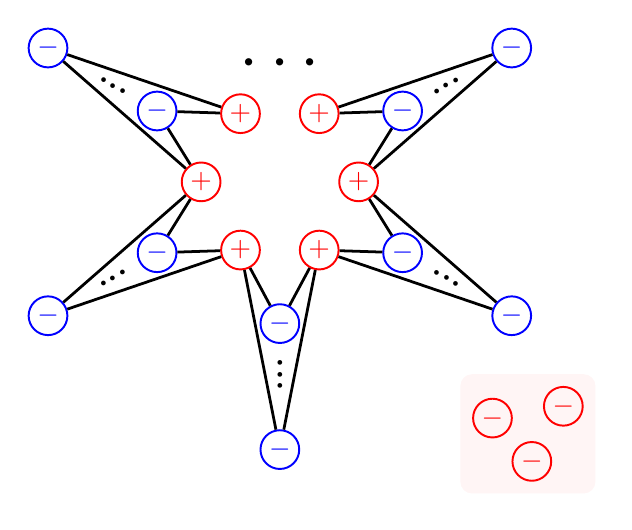
\begin{tikzpicture}
            \depstyle{cjob}{circle, line width=0.7pt, draw=black!80, minimum size=14pt, inner sep=0pt}
            \depstyle{carrow}{-, line width=1pt}
            \depstyle{cbox-red}{fill=red!4, rounded corners, draw=red!4}

            % Пестик:
            \foreach \i/\t in {60/1, 120/2, 180/3, 240/4, 300/5, 0/6} {
                \begin{scope}[rotate={\i + 30}]
                    \node[cjob, color=red] (plus-\t) at (0, 1) {$+$};
                \end{scope}
            }

            % Лепестки:
            \foreach \i/\l/\r in {60/6/1, 120/1/2, 180/2/3, 240/3/4, 300/4/5} {
                \begin{scope}[rotate=\i]
                
                    \node[cjob, color=blue] (sad1) at (0, 1 + 1*0.8) {$-$};
                    \draw[carrow] (sad1) -- (plus-\l);
                    \draw[carrow] (sad1) -- (plus-\r);
                    
                    \node[rotate=\i, font=\fontsize{20}{0}\selectfont] (sad2) at (0, 1 + 2*0.8 - 0.05) {$\vdots$};
                    
                    \node[cjob, color=blue] (sad3) at (0, 1 + 3*0.8) {$-$};
                    \draw[carrow] (sad3) -- (plus-\l);
                    \draw[carrow] (sad3) -- (plus-\r);
                \end{scope}
            }

            % Свободные негативные вершниы:
            \begin{scope}[shift=({3, -3.25})]
                \path (-0.3 - 0.4, -0.3 - 0.4) node (a1) {};
                \path (0.6 + 0.4, 0.4 + 0.4) node (a2) {};
                % \path (-0.3 - 0.4 + 0.8, 0.4 + 0.4 + 0.2) node (u1)[texto] {\textit{Свободные вершины}};
                \path[cbox-red] (a1) rectangle (a2);
                
                \node[cjob, color=red] (sad) at (0.2, -0.3) {$-$};
                \node[cjob, color=red] (sad) at (0.6, 0.4) {$-$};
                \node[cjob, color=red] (sad) at (-0.3, 0.25) {$-$};
            \end{scope}

            \node[font=\fontsize{40}{0}\selectfont] (plus-dots) at (0, 1.5) {$\cdots$};
            % \node[] (plus-dots-a) at (0, 2.7) {$\displaystyle a = \left\lceil \frac{n}{k} \right\rceil$;};

            % \node[font=\fontsize{20}{0}\selectfont] at (1.4, -1.125) {$G'$};
        \end{tikzpicture}
    }
    \caption{Пример графа. Используются циклы. Картинка равномерно уменьшена чтобы занимала меньше места.}
\end{figure}

\begin{figure}[H]
    \centering
    \small
    \begin{dependency}
        \begin{deptext}[column sep=0em]
            В \& некоторых \& {}[\textbf{случаях}] \& {}{[\textbf{это}]} \& \underline{\underline{может}} \& привести \& к \& нежелательным \& {}[\textbf{последствиям}]. \\
        \end{deptext}
        \deproot{5}{root}
        \depedge{3}{1}{case}
        \depedge{3}{2}{det}
        \depedge{5}{3}{obl}
        \depedge{5}{4}{nsubj}
        \depedge{5}{6}{xcomp}
        \depedge{6}{9}{obl}
        \depedge{9}{8}{amod}
        \depedge{9}{7}{case}
    \end{dependency}
    \caption{Пример рисунка, выполненного через библиотеку tikz-dependency.}
    \label{fig:example fig 5}
\end{figure}

\begin{figure}[h]
    % Не ставьте лишних пустых строк тут: они разобьют картинку на абзацы.
    \centering
    \begin{subfigure}[t]{0.45\textwidth}
        \centering
        \resizebox{0.8\textwidth}{!}{
            \begin{tikzpicture}
                \begin{axis}[
                    axis lines = middle,
                        xlabel = {$t$},
                        ylabel = {$x(t)$},
                        xmin = -1, xmax = 4,
                        ymin = 0, ymax = 2,
                        minor tick num = 2
                    ]
                    \addplot[blue] coordinates {
                        (-1,0) (0,0) (0,1) (4,1)
                    };
                    \addlegendentry{$g(t)$}
                    \addplot[red, samples=150] {(1 - 0.5*e^(-x)*(cos(deg(10*x) + sin(deg(10*x))))) * (x > 0 ? 1 : 0)};
                    \addlegendentry{$x(t)$}
                \end{axis}
            \end{tikzpicture}
        }
        \caption{Нарисованный средствами тех-а график затухающего колебания.}
        \label{fig:example subfig 1}
    \end{subfigure}
    \hfill % Эта команда заполняет всё доступное пустое пространство пробелами.
    \begin{subfigure}[t]{0.45\textwidth}
        \centering
        \resizebox{0.6\textwidth}{!}{
            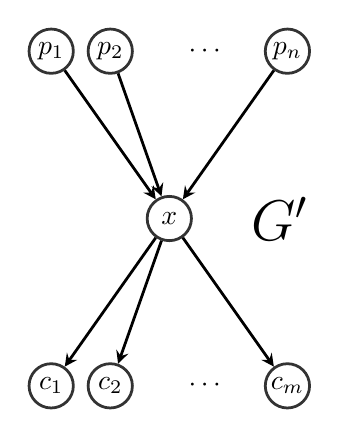
\begin{tikzpicture}
                \depstyle{cjob}{circle, line width=1pt, draw=black!80, fill=white, minimum size=16pt, inner sep=0pt}
                \depstyle{carrow}{-stealth, line width=1pt}
                % Граф. Задаём вершины и связи между ними:
                \node[cjob] (x)      at (0, -1.125) {$x$};
    
                \node[cjob] (p1)     at (-0.75*2, 1)    {$p_1$};
                \node[cjob] (p2)     at (-0.75, 1) {$p_2$};
                \node[    ] (pdots)  at (0.75 - 0.3, 1) {$\cdots$};
                \node[cjob] (pn)     at (0.75*2, 1)     {$p_n$};
                \draw[carrow] (p1) -- (x);
                \draw[carrow] (p2) -- (x);
                \draw[carrow] (pn) -- (x);
    
                \node[cjob] (c1)     at (-0.75*2, -3.25)    {$c_1$};
                \node[cjob] (c2)     at (-0.75, -3.25) {$c_2$};
                \node[    ] (cdots)  at (0.75 - 0.3, -3.25) {$\cdots$};
                \node[cjob] (cm)     at (0.75*2, -3.25)     {$c_m$};
                \draw[carrow] (x) -- (c1);
                \draw[carrow] (x) -- (c2);
                \draw[carrow] (x) -- (cm);
                
                \node[font=\fontsize{20}{0}\selectfont] at (1.4, -1.125) {$G'$};
            \end{tikzpicture}
        }
        \caption{Нарисованный средствами тех-а граф.}
        \label{fig:example subfig 2}
    \end{subfigure}
    \caption{Общая подпись с общей ссылкой \texttt{fig:example subfigs}. На под-рисунки можно ссылаться так: \ref{fig:example subfig 1}, \ref{fig:example subfig 2}.}
    \label{fig:example subfigs}
\end{figure}

В одной \verb!figure! или \verb!table! могут быть несколько объектов со своими подписями. Для этого используются окружения \verb!subfigure!. Одним из их аргументов задаётся ширина: например, два под-рисунка ниже имеют ширину $0.45$ от ширины страницы. Между окружениями стоит команда \verb!\hfill!, которая заполняет пространство между под-рисунками пробелами. На под-рисунки так же можно ссылаться: \ref{fig:example subfig 1}.




\section{Ссылки на объекты в тексте и источники}\label{section:references}

Ссылка на картинку, формулу и другие объекты происходит при помощи команды  \verb!\ref!: см. рис. \ref{fig:example fig 1}. На ссылку можно кликнуть и перейти к объекту, на который она ссылается. Ссылка может быть как до объекта, так и после него. Обычно, для удобства, идентификатор начинают с префикса <<\verb!fig:!>> для рисунков, <<\verb!tab:!>> для таблиц, <<\verb!eq:!>> для формул, для <<\verb!section:!>> для разделов, <<\verb!th:!>> для теорем и так далее. Пример ссылки на раздел: см. раздел \ref{section:references}. Ссылаться на сноску можно как обычно: см. сноску \ref{footnote:example} или, как вариант, меткой в верхнем индексе, как это происходит обычно\footref{footnote:example}. Если ссылка не правильная, компилятор выдаст предупреждение, а ссылка будет выглядеть так: \ref{wrong ref}.

По условиям гост-а, на каждую картинку и таблицу должна присутствовать в тексте хотя бы одна ссылка.

Обратите внимание, что цветовые обозначения всех ссылок не допускаются в ВКР\footnote{Потому что основная форма текста ВКР -- печатная. \label{footnote:example}} и были убраны здесь.

Интернет-ссылки могут быть оформлены в двух вариантах:
\begin{enumerate}
    \item обычная ссылка: \url{https://www.google.com/};
    \item \href{https://www.google.com/}{текстовая ссылка (здесь, в ВКР, не выделяется цветом)}.
\end{enumerate}
Обе версии кликабельны.

Информация об цитируемых источниках хранится в файлах формата \verb!*.bib!. В этом проекте есть пример такого файла \verb!references.bib!. Похож на формат \verb!json!, но им не является. Заполняйте как можно больше полей там. Сразу готовую запись можно получить прямо в Google Scholar или, часто, на страницах статьей на других ресурсах (см. рис. \ref{fig:scholar}). Описание статей начинается с заголовка \verb!@article!, для источников других видов предусмотрены другие заголовки, например \verb!@online! для интернет-страниц.

\begin{figure}[h]
    \centering
    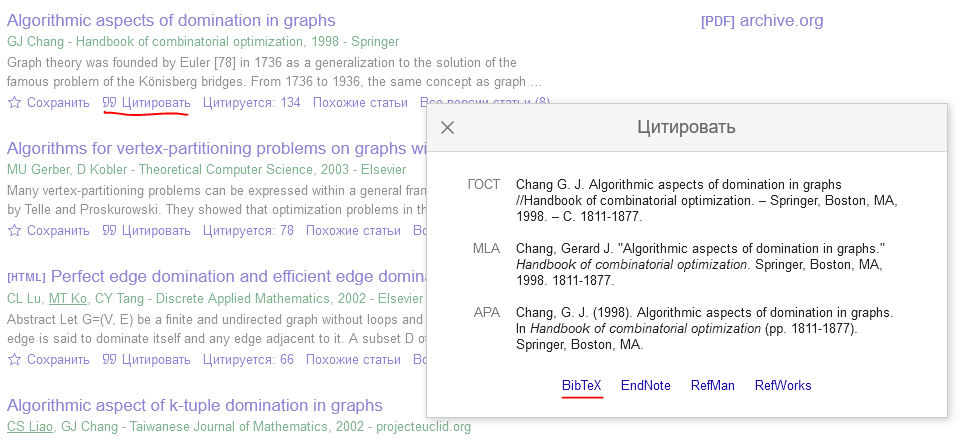
\includegraphics[scale=0.5]{img/scholar.png}
    \caption{Как получить bib-цитату на источник в Google Scholar.}
    \label{fig:scholar}
\end{figure}

Ссылка на источник происходит при помощи команды \verb!\cite!: \cite{duportail:alu}. В качестве единственного аргумента указывается идентификатор источника в одном из файлов \verb!*.bib!. Можно указать несколько источников: \cite{duportail:alu, althusser:iia, husserl:pd}, с \verb!\ref! так нельзя. В списке источников отображаются только те источники, на которых есть хотя бы одна ссылка. Если всё-же нужно что бы он там появился без единой ссылки, можно использовать команду \verb!\nocite! в любом месте программы, как под этим абзацем. Если ссылка не правильная, компилятор выдаст предупреждение, а ссылка будет выглядеть так: \cite{wrong ref}.

\nocite{duportail:alu}
\nocite{althusser:iia}
\nocite{husserl:pd}
\nocite{husserl:sbe}


\subsubsection{О сортировке источников}

Существует следующая \textit{рекомендация} по отображению списка источников: русскоязычные источники должны стоять сверху, а уже потом все остальные. Автоматически так сделать не получиться. Однако, в данном шаблоне настроено так, что источники, у которых указан параметр \verb!language = {russian}! в \verb!*.bib!-файле, будет стоять выше остальных. Если вы хотите следовать этой рекомендации, вам необходимо указывать вручную этот параметр для каждого русскоязычного источника.




\section{Псевдо-код и код}

Псевдокод в ВКР рекомендуется оформлять на русском языке. Больше информации по псевдо-коду можете найти по ссылке: \url{https://harrix.dev/blog/2013/algorithmicx-cyrillic/}.

\begin{algorithm}
    \begin{algorithmic}[1]
        \State $X=45$
        \For{\textbf{от} $i=0$ \textbf{до} 5}
            \State $X=X-2$
            \State \Call {Find}{$X$}
            
            \While{$Y_2<5$}
                \If{$quality\ge 9$}
                    \State $a\gets \mathtt{good}$
                \ElsIf{$quality\ge 7$}
                    \State $a\gets \mathtt{medium}$
                \Else
                    \State $a\gets \mathtt{unusable}$
                \EndIf
            \EndWhile
            
            \State \Return $X$
        \EndFor
    \end{algorithmic}
    \caption{Пример алгоритма}
    \label{alg:examples}
\end{algorithm}

\begin{algorithm}
    \begin{algorithmic}[1]
        \Require $x \ge 0$

        \While{$x < 2^10$}
            \State $x \gets \mathtt{Pow}(x, 2)$
        \EndWhile
        \State $\mathtt{Prtin}(x)$
        
        \Statex
            
        \Procedure{Print}{$x \in \mathbb R$}
            \State Вывести число $x$ в \verb!std::cout!
        \EndProcedure
        
        \Statex
        
        \Function{Pow}{$a, b \in \mathbb R$}
            \State \Return $a^b$
        \EndFunction
    \end{algorithmic}
    \caption{Пример алгоритма 2}
    \label{alg:examples2}
\end{algorithm}

\newpage
Можно вставлять код. Есть вариант однострочный: \lstinline[language=Python]{array: List = [1, 2, 3]}. Для варианта с многострочным блоком кода необходимо следить за тем, что бы все строки помещались в блок:
\begin{lstlisting}[language=Python]
df1 = pd.DataFrame({
   'имя': ['Солнце', 'Сириус', 'Альдебаран', None],
   'радиус': [1, None, 3, None],
   'цвет': ['жёлтый', 'синий', None, None]
})
   
# Удалить строки где есть хотя-бы один пропуск:
df1 = df1.dropna()
# или
df1 = df1.dropna(axis=0, how='any')
    #    имя     радиус  цвет
    # 0  Солнце  1.0     жёлтый

# Удалить только полностью пустые строки:
df1 = df1.dropna(axis=0, how='all')
    #    имя         радиус  цвет
    # 0  Солнце      1.0     жёлтый
    # 1  Сириус      NaN     синий
    # 2  Альдебаран  3.0     None
\end{lstlisting}

Можно так же вставлять код из файла:
\lstinputlisting[language=Python]{code/code_example.py}


\end{document}